%% Ankur Sinha

%% packages %%
% support for coloured text
\usepackage{color}
% IPA
\usepackage{tipa}
\usepackage[scale=2]{ccicons}
\usepackage{amssymb}
\usepackage{tikz}
\usetikzlibrary{arrows.meta, arrows}
\usepackage{jneurosci}
\usepackage{subfig}
\usepackage[T1]{fontenc}
\usepackage[utf8]{inputenc}
\usepackage[style=nature,backend=biber,autocite=footnote]{biblatex}
\addbibresource{/home/asinha/Documents/01_Readables/00_research_papers/masterbib.bib}
% Use opensans
\usepackage[default,osfigures,scale=0.95]{opensans}
% for strike through
\usepackage[normalem]{ulem}
% links, urls, refs
\definecolor{links}{HTML}{2A1B81}
% Fedora blue for the theme
\definecolor{FedoraBlue}{HTML}{2A1B81}
\usepackage{hyperref}
\hypersetup{colorlinks,linkcolor=Green,urlcolor=links}
% graphics
\usepackage{graphicx}
% algorithm
\usepackage{algorithmic}
\usepackage{textcomp}
\usepackage{wrapfig}
\usepackage{textgreek}
\usepackage{euler}

% beamer theme
% use defaults for theme
\usetheme[numbering=fraction]{metropolis}
\usefonttheme[onlymath]{serif}
\setbeamerfont{footnote}{size=\tiny}
\setbeamerfont{caption}{size=\tiny}
\setbeamercolor{alerted text}{fg=Green}

% Not needed in metropolis, but in general footnote citation fixes: https://tex.stackexchange.com/questions/44217/how-can-i-stop-footcite-from-hijacking-my-beamer-columns
% how to use multiple references to the same footnote: https://tex.stackexchange.com/questions/27763/beamer-multiple-references-to-the-same-footnote

%% title %%
\title{Investigating the activity dependent dynamics of synaptic structures using biologically realistic modelling of peripheral lesion experiments}
\subtitle{Discussion of my Ph.D. research}
\author[Ankur Sinha]{Ankur Sinha}
\date{29/03/2019}

%% document begins %%
\begin{document}

% title frame %%
\begin{frame}
  \titlepage{}
\end{frame}

%% Three slides for 5 minutes seems good
%% So, 30 slides at most for 50 minutes
\section{Context}
\begin{frame}[c]{Plasticity while maintaining stability}
  \begin{figure}[h]
    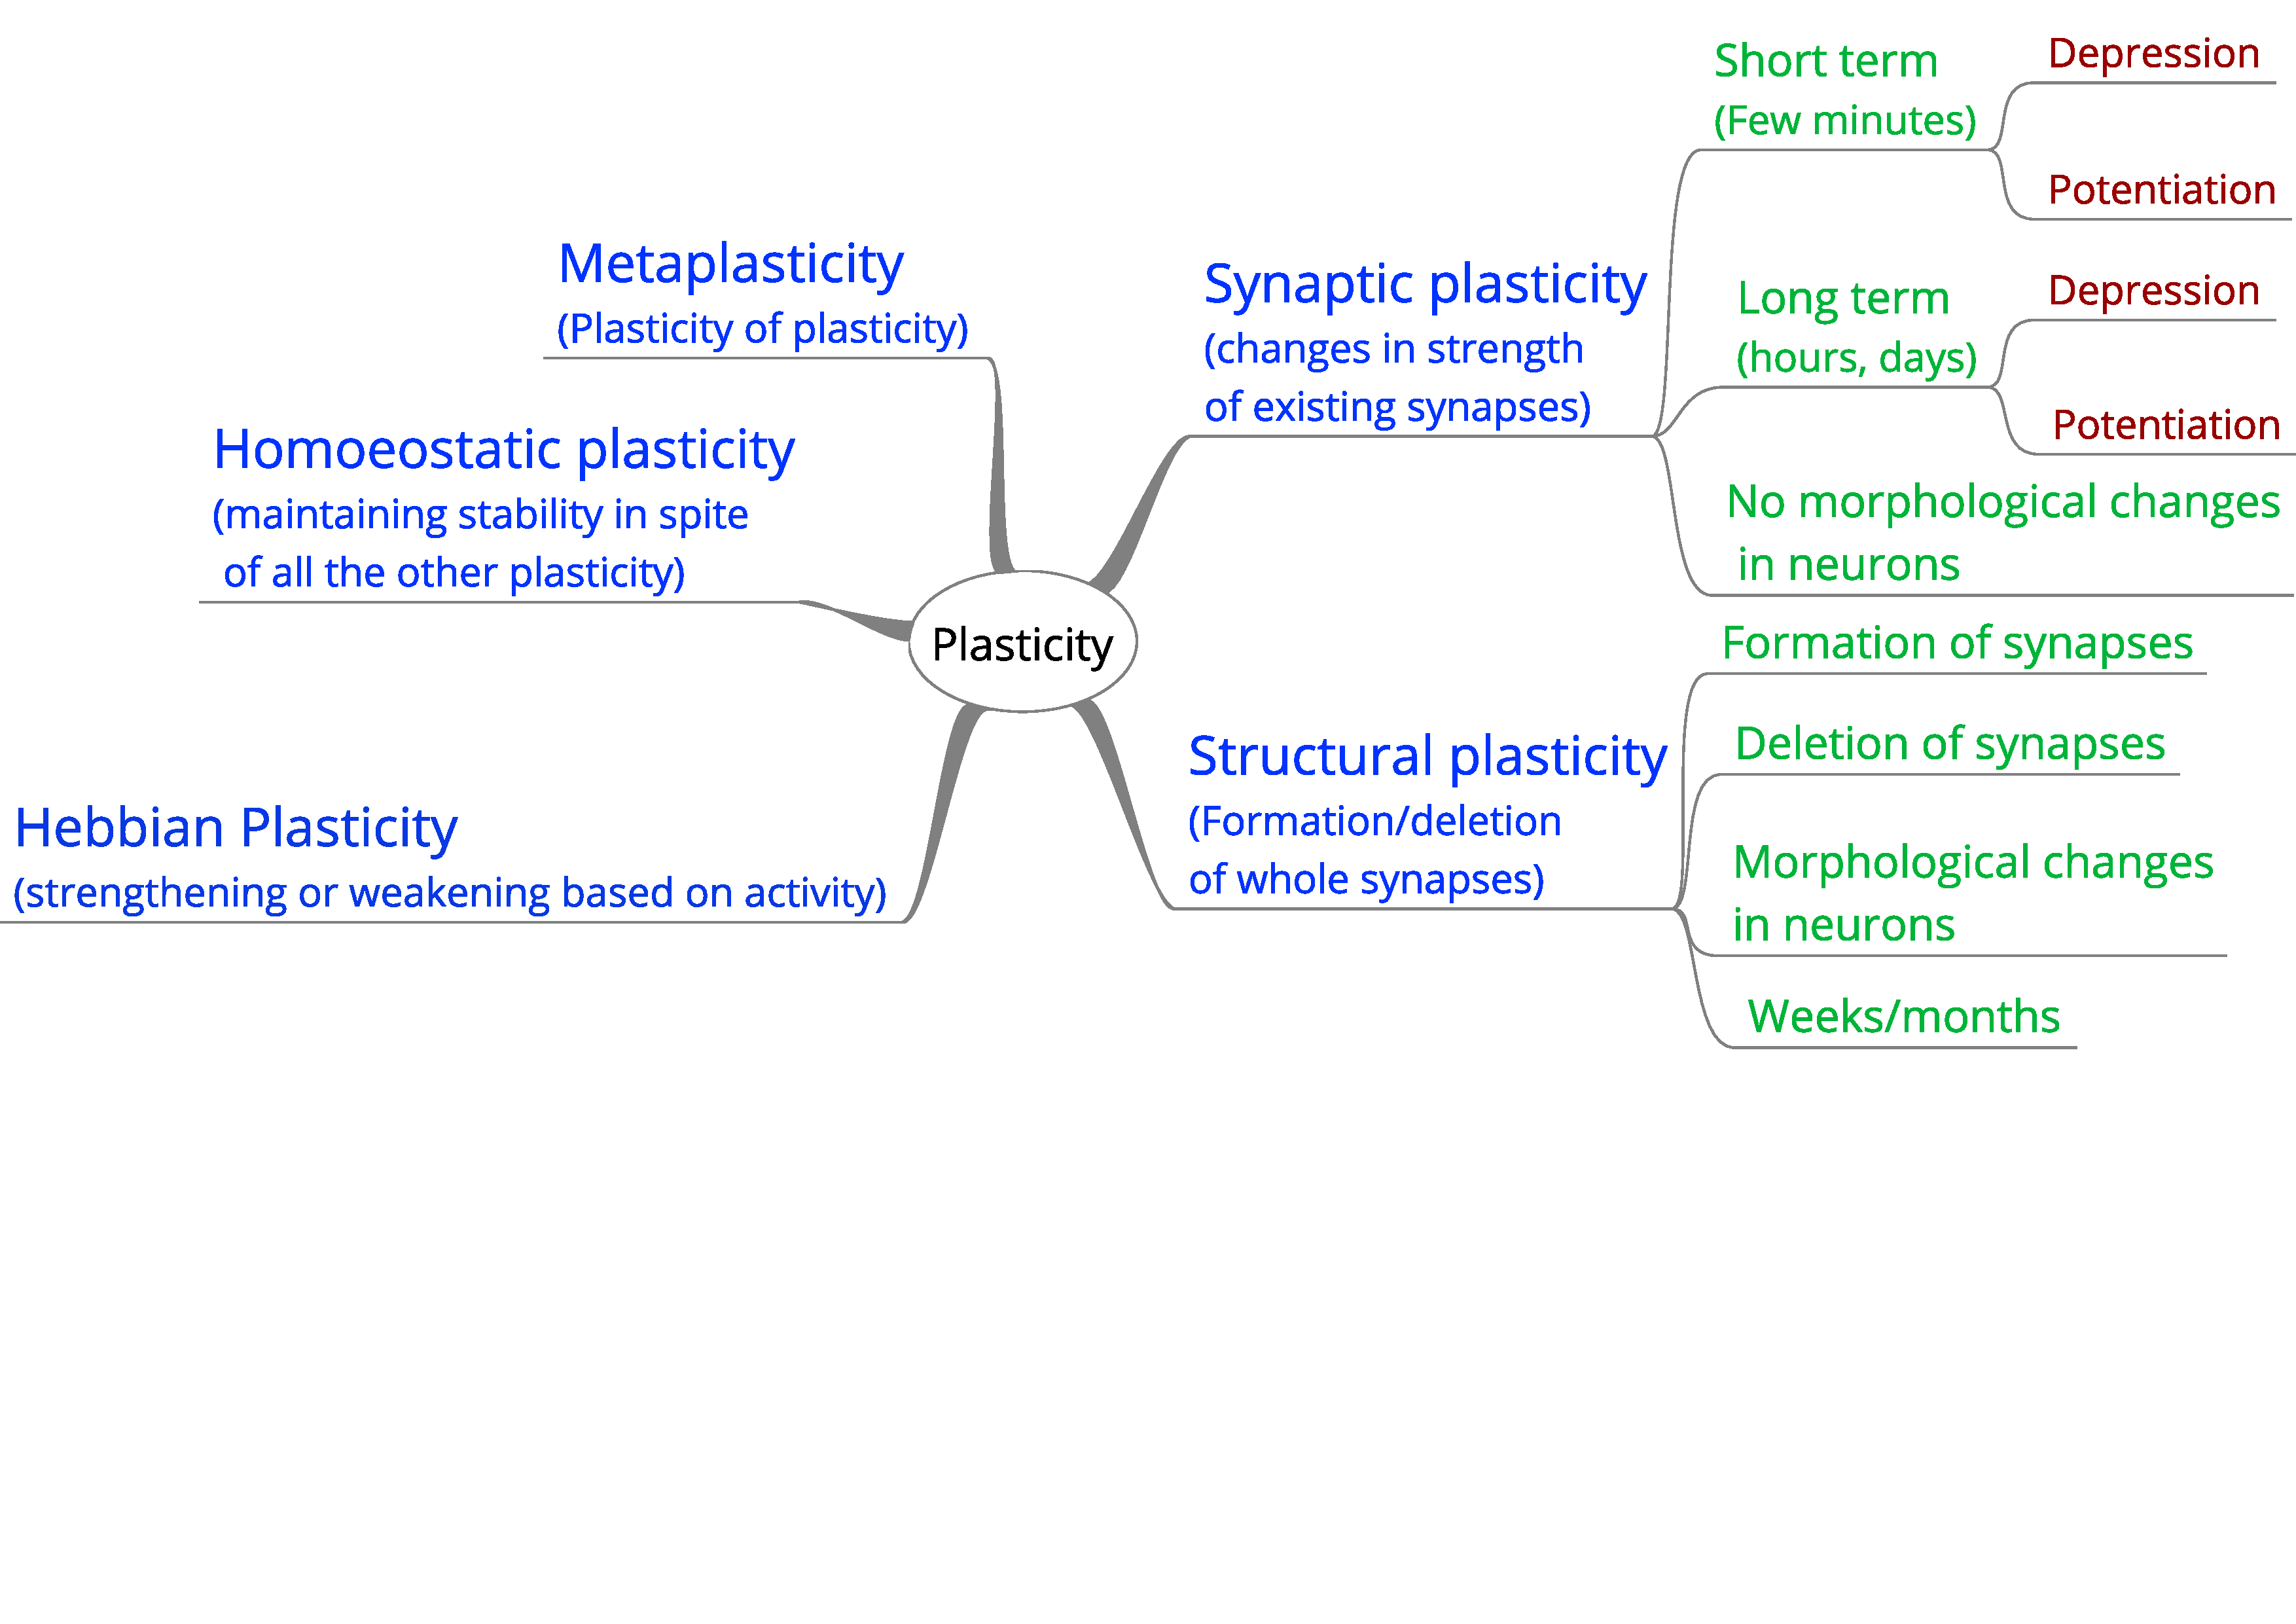
\includegraphics[width=1.05\linewidth]{99_images/Plasticity.pdf}
  \end{figure}
  \note[item]{We know there are multiple plasticity mechanisms active all at once. Hebbian plasticity underlies learning, but de-stabilises networks. Homeostatic plasticity ensures that even when learning occurs, the network remains in a stable state}
  \note[item]{Generally, though, when we speak of these, we refer to synaptic plasticity only. But, lots of evidence now confirms that, in fact, structural plasticity is active in the adult brain. So not only are synaptic weights changing, the connectivity of networks is changing too!}
  \note[item]{So, it isn't hard to imaging how if changes in synaptic strengths makes plasticity-stability an issue, how the removal and formation of whole synapses would have a much larger effect to plasticity-stability.}
  \note[item]{For the purpose of our analysis, we do not consider the modulation of synaptic strengths as structural plasticity (even though it is).}
\end{frame}
\begin{frame}[c]{Synaptic structures are dynamic in the adult brain}
  \note[item]{In the adult brain, now that we have the tech to look in at the microscopic structures that form synapses, we see that these are highly dynamic. They sprout and retract, forming and removing synapses. However, this must happen in a way that the brain remains functional: so, are their Hebbian and Homeostatic components of structural plasticity too?}
  \tiny{
  \begin{enumerate}
    \item \fullcite{Chen2011}
    \item \fullcite{Marik2010}
    \item \fullcite{Marik2014}
    \item \fullcite{Stettler2006}
    \item \fullcite{Gogolla2007}
    \item \fullcite{Holtmaat2005}
    \item \fullcite{Chen2012}
    \item \fullcite{Trachtenberg2002}
    \item \fullcite{Villa2016}
  \end{enumerate}
  }
\end{frame}
\begin{frame}[c]{Evidence of homeostatic structural plasticity: lesion studies}
  \note[item]{The simplest way of studying homeostatic mechanism is to nudge the network out of its stable state. Lesion studies have, for a long time, observed structural changes after peripheral lesioning. A peripheral lesion is where you dont destroy the network itself, but you disrupt the input to it---we'll come to this in detail later.}
  \tiny{
    \begin{enumerate}
      \item \fullcite{Wall1984}
      \item \fullcite{Rasmusson1982}
      \item \fullcite{Rajan1993}
      \item \fullcite{Pons1991}
      \item \fullcite{Allard1991}
      \item \fullcite{Darian-Smith1994}
      \item \fullcite{Darian-Smith1995}
      \item \fullcite{Florence1998}
      \item \fullcite{Heinen1991}
    \end{enumerate}
  }
\end{frame}
\begin{frame}[c]{Detailed lesion experiments to study synaptic structures}
  \note[item]{With more tech, neuroscientists have been able to mark, track, and analyse micro-structures that are involved in synapses: boutons, spines, dendritic trees. So, there's recently quite a bit of data from these.}
  \tiny{
    \begin{enumerate}
      \item \fullcite{Chen2011}
      \item \fullcite{Marik2010}
      \item \fullcite{Yamahachi2009}
      \item \fullcite{Hickmott2005}
      \item \fullcite{Keck2008}
      \item \fullcite{Keck2011}
      \item \fullcite{Trachtenberg2002}
    \end{enumerate}
  }
\end{frame}
\begin{frame}[c]{Experimental protocol I}
  \note[item]{The protocol is pretty standard. Here, for a study in the visual cortex, the retinal field of a rat or a mouse is mapped.}
  \begin{columns}
    \begin{column}{0.5\textwidth}
      \centering
      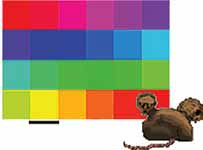
\includegraphics[width=0.8\textwidth]{99_images/keck-1-1a}%chktex 8
    \end{column}
    \begin{column}{0.5\textwidth}
      \centering
      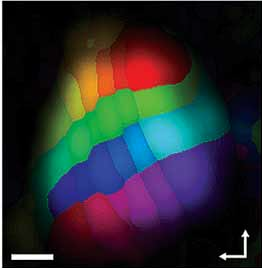
\includegraphics[width=0.8\textwidth]{99_images/keck-1-1c}%chktex 8
    \end{column}
  \end{columns}
  \footnotetext[1]{\fullcite{Keck2008}}
\end{frame}
\begin{frame}[c]{Experimental protocol II:\ after peripheral lesion}
  \note[item]{Then, a part of the retina is lesioned. This cuts off inputs to a part of the visual cortex, as shown in the first figure. This forms the Lesion Projection Zone (LPZ). By repeated imaging of the region over months, the reorganisation of the network is tracked.}
    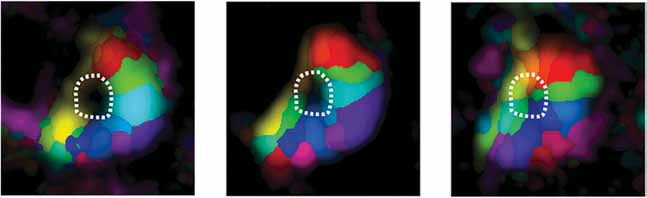
\includegraphics[width=\textwidth]{99_images/keck-1-2c}%chktex 8
    \footnotetext[1]{\fullcite{Keck2008}}
\end{frame}
\begin{frame}[c]{What we know from these experiments}
  \note[item]{So, if this a simple schematic, of the regions around the LPZ, this is what we know from these studies.}
  \begin{columns}
    \begin{column}{0.3\textwidth}
      \centering
      \def\radiuscircle{0.6cm}
\begin{tikzpicture}[scale=0.8, transform shape]
  \fill [fill=black, thick, opacity=0.10] (0,0) rectangle ++(5,7.5);
  \node [below, black] at (3.5, 1.0){Other};

  \fill [cyan, opacity=1.0] (2.5, 3.5) circle (3.0*\radiuscircle);
  \draw [cyan, very thick] (1.5, 1.0)--(2.5, 3.5);
  \node [below, cyan] at (1.5, 1.0){Peri LPZ};

  \fill [black, opacity=1.0] (2.5, 3.5) circle (2.0*\radiuscircle);
  \draw [black, very thick] (1.5, 6.0)--(2.5, 3.5);
  \node [above, black] at (1.5, 6.0){LPZ B};

  \fill [green, opacity=1.0] (2.5, 3.5) circle (\radiuscircle);
  \draw [green, very thick] (3.5, 6.0)--(2.5, 3.5);
  \node [above, green] at (3.5, 6.0){LPZ C};

\end{tikzpicture}

    \end{column}
    \pause{}
    \begin{column}{0.6\textwidth}
      \begin{itemize}
        \item Massive disinhibition in the LPZ\@.
        \item Ingrowth of excitatory synapses from the peri-LPZ to the LPZ\@.
        \item Outgrowth of inhibitory synapses from the LPZ to the peri-LPZ\@.
      \end{itemize}
    \end{column}
  \end{columns}
\end{frame}
\begin{frame}[c]{Computational modelling:\ MSP I}
  \note[item]{Computational modelling stems from evidence from decades years ago. It was established that outgrowth depends on the change in the Calcium concentration in neurons.}
  \note[item]{So, in this figure, we see that a neurotransmitter causes a change in the Calcium of the neuron, and that causes some change in its outgrowth.}
  \note[item]{What this suggests, is that there's an optimal level of Calcium for neurons to have \enquote{normal} growth.}
  \note[item]{Based on this, Butz and van Ooyen came up with a framework for modelling structural plasticity. In this, they modelled the rate of change of synaptic elements as a Gaussian function of the neuron's Calcium concentration.}
  \begin{columns}
    \begin{column}{0.5\textwidth}
      \centering
      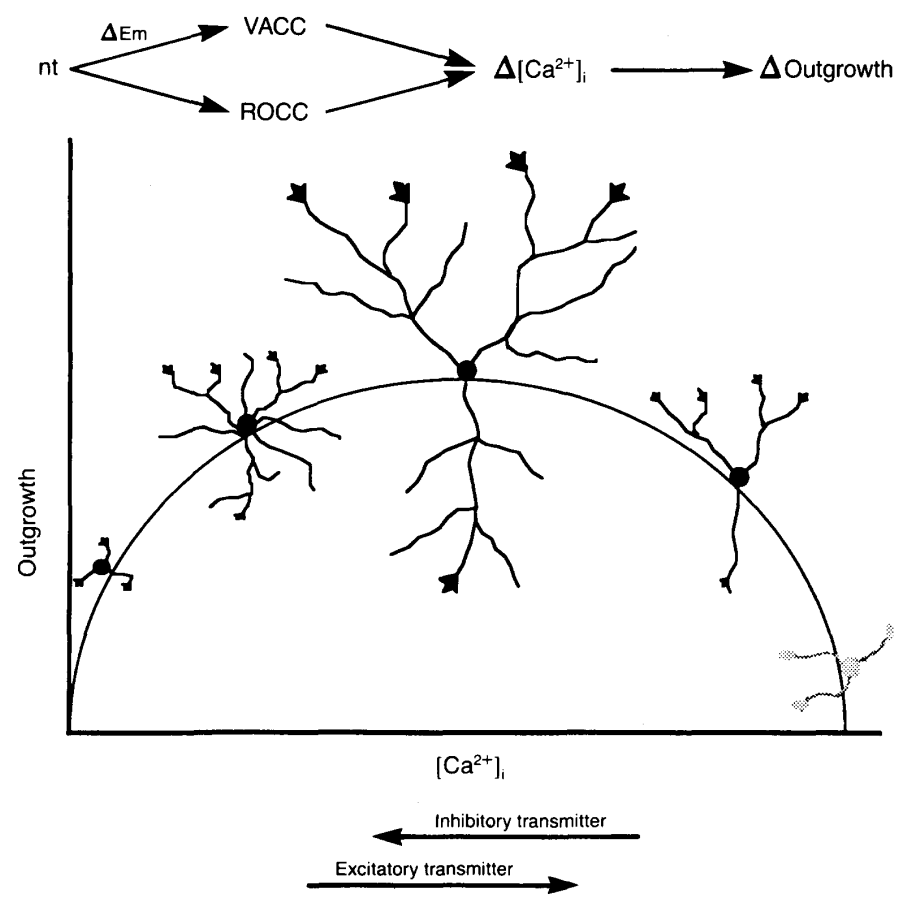
\includegraphics[width=0.9\textwidth]{99_images/lipton1989.png}%chktex 8
    \end{column}
    \begin{column}{0.5\textwidth}
      \centering
      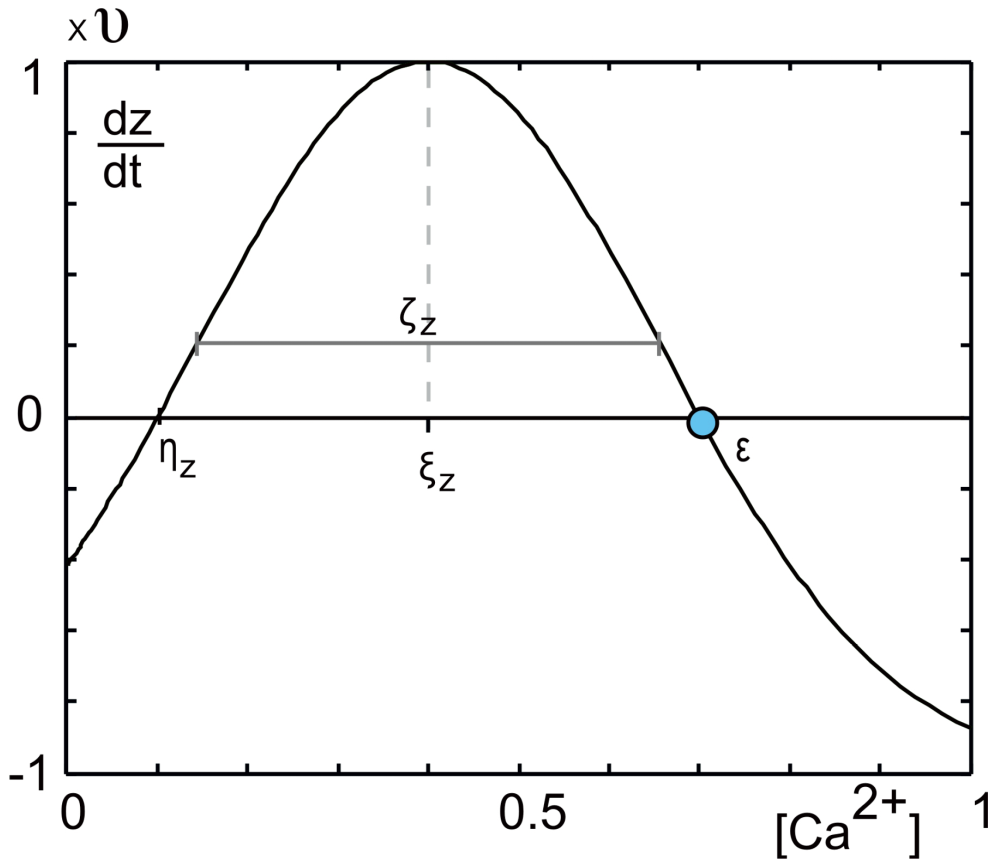
\includegraphics[width=0.9\textwidth]{99_images/growth-curve-general.png}%chktex 8
    \end{column}
  \end{columns}
  \footnotetext[2]{\fullcite{Lipton1989}}
  \footnotetext[3]{\fullcite{Butz2013}}
\end{frame}
\begin{frame}[c]{Computational modelling:\ MSP II}
  \begin{columns}
    \begin{column}{0.6\textwidth}
      \begin{itemize}
        \item Synaptic structures (\(z\)): excitatory \alert{and} inhibitory post-synaptic, excitatory \alert{or} inhibitory pre-synaptic elements.
        \item New synapses form when \alert{free} plugs are available: (\(z > z_{conn}\))
        \item Synapses are deleted if: (\(z < z_{conn}\))
      \end{itemize}
    \end{column}
    \begin{column}{0.5\textwidth}
      \centering
      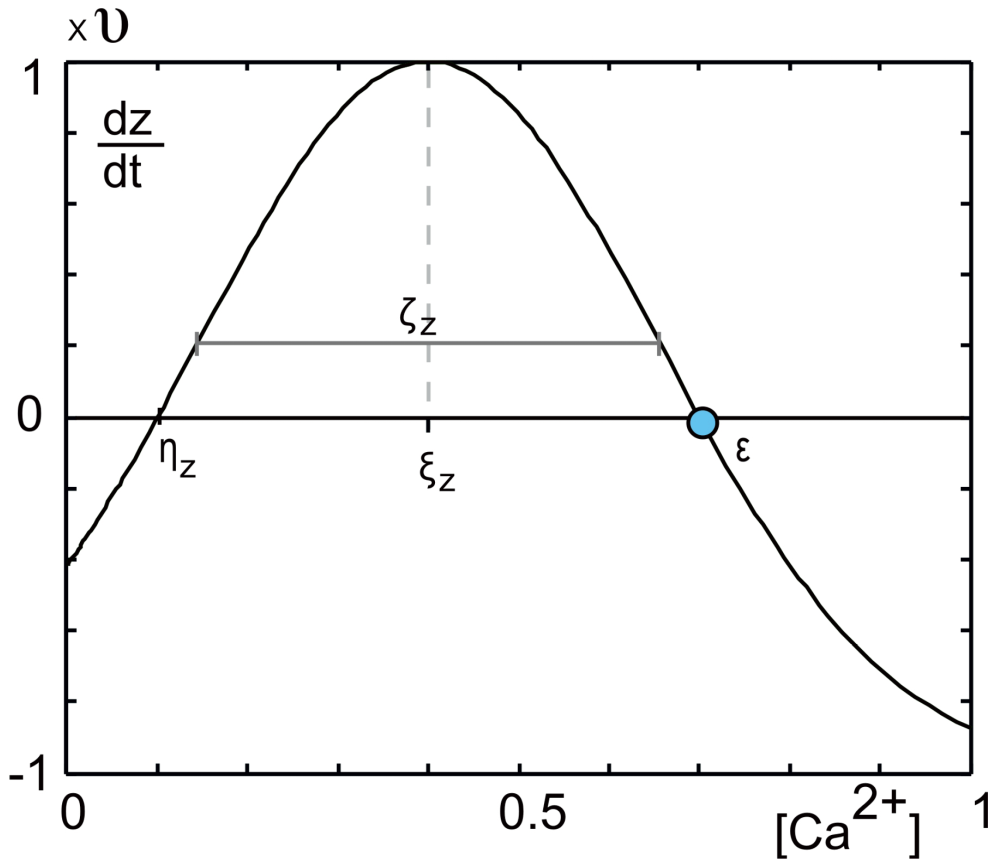
\includegraphics[width=0.9\textwidth]{99_images/growth-curve-general.png}%chktex 8
    \end{column}
  \end{columns}
\end{frame}
\begin{frame}[c]{Computational modelling II}
  \centering
  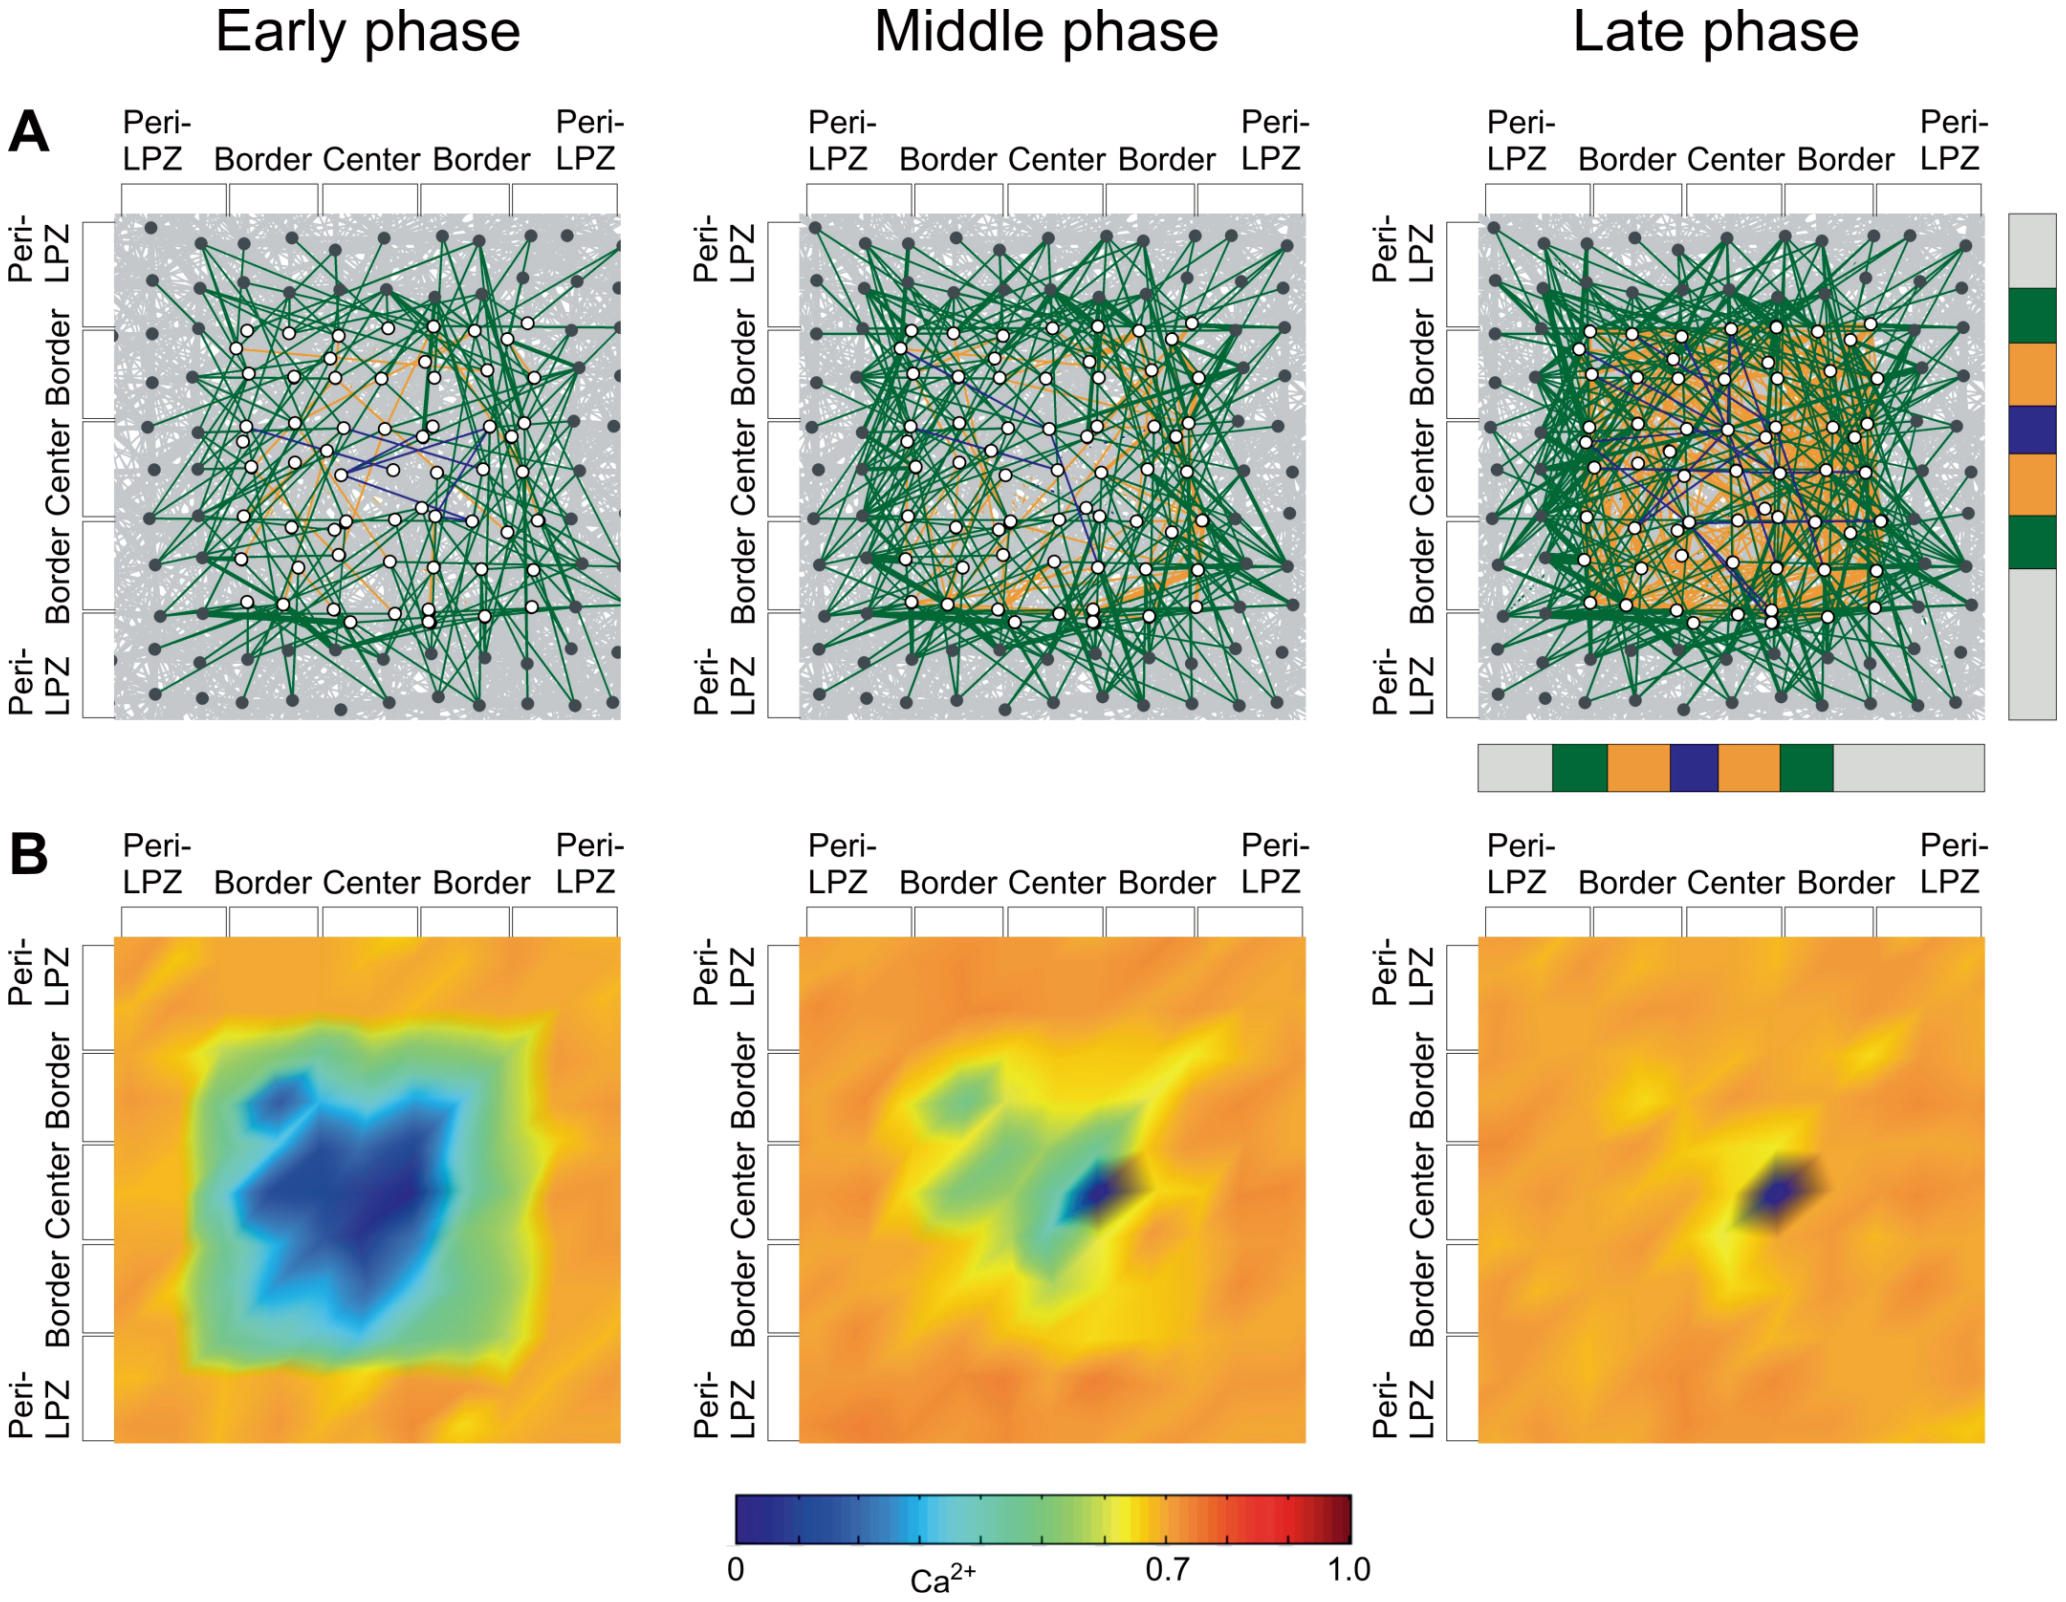
\includegraphics[width=0.7\textwidth]{99_images/butz3.png}
  \footnotetext[2]{\fullcite{Butz2013}}
\end{frame}

\section{Methods}
\section{Results and discussion}
\end{document}

